\chapter{能量习题精讲}
\begin{calculate}
  1.一质量为$0.3kg$的弹性小球,在光滑的水平面上以$6m/s$的速度垂直撞在墙上,碰撞后小球沿相反方向运动,反弹后的速度大小与碰撞前速度的大小相同,则碰撞后小球速度变化量的大小$\Delta x$和碰撞过程中墙地小球做功的大小W.

  a. $\Delta x=12m/s$ \qquad $W=0$

  e.设末速度方向为正,则初速度为$v_0=-6m/s$,末速度为$6m/s$,则
  \[
    \Delta v=v-v_0=12m/s
  \]
  由动能定理得
  \[
    W=\frac{1}{2}mv^2-\frac{1}{2}mv_0^2=0
  \]


  2.一质量为$m$的小球,用长为$l$的轻绳悬挂于$O$点.小球在水平拉力$F$的作用下,从平衡位置$P$点很缓慢地移动到$Q$点,如
<:
\begin{tikzpicture}
  \draw [color=white,pattern=north west lines] (-0.5,0) rectangle (0.5,0.2);
  \draw (-0.5,0)--(0.5,0); 
  \draw[dashed] (0,0)--(0,-2);
  \draw (0,-2.2) circle [radius=0.2];
  \draw (0,0)--(300:2);
  \draw (300:2.2) circle [radius=0.2];
  \draw[->,>=stealth] (300:2.2)++(0.2,0)--++(1,0) node [anchor=south]{\small $F$};
  \draw (270:0.5) arc (270:300:0.5);
  \draw (285:0.7) node {\small $\theta$};
  \draw (-0.4,-2.2) node {\small $P$};
  \draw (290:2.2) node {\small $Q$};
  \draw (310:1.4) node {\small $l$};
\end{tikzpicture}
:>所示,则拉力F所做的功为多少?

a.$mgl(1-\cos\theta)$

e.此题将小球缓慢移动,所以可以认为每时每刻都处于静止状态.即P点和Q点的速度都是0.从P点到Q点由动能定理得
\[
  -mgl(1-\cos\theta)+W_F=0-0
\]
解得
\[
  W_F=mgl(1-\cos\theta)
\]

3.如<:
\begin{tikzpicture}
  \draw [color=white,pattern=north west lines] (0,0) rectangle (2,-0.2); 
  \draw (0,0)--(2,0);
  \draw (0,0)--(150:1.5);
  \draw[rotate=150] (1.2,0) rectangle (1.5,-0.3);
  \draw[dashed](-1.5,0)--(0,0);
  \draw[<->,>=stealth](150:1.45)--(-1.2557,0);
  \draw (-1.3,0.35) node [anchor=east]{\small $h$};
  \draw (150:1.5) node [anchor=east] {\small $A$};
  \draw (0,-0.2) node [anchor=north] {\small $B$};
  \draw (2,-0.2) node [anchor=north] {\small $C$};
\end{tikzpicture}
:>所示物体从高h的斜面顶端A由静止滑下,到斜面底端后又沿水平面运动到C点面停止.要使这个物体从C点沿原路返回到A.则在C点处物体应具有的速度大小$v_0$至少是多少?

a.$2\sqrt{gh}$

e.物体从A到C的过程中,A点速度为零,C点速度为零,则由动能定理得
\[
  mgh+W_f=0-0
\]
解得
\[
  W_f=-mgh
\]
物体从C到A的过程中,设C速度为$v_0$,则恰好回到A点时$v_0$最小,则此时$A$点速度为0,同时此过程摩擦力也做负功,大小与从A到C摩擦力做功大小相同.所以由动能定理得
\[
  -mgh+W_f=0-\frac{1}{2}mv_0^2
\]
将$W_f=-mg$代入解得
\[
  v_0=2\sqrt{gh}
\]

4.一架喷气式飞机,质量为$m=5\times10^3kg$,起飞过程中从静止开始滑跑的路程为$s=5.3\times10^2m$时,达到起飞的速度$v=60m/s$,在此过程中飞机受到的平均阻力是飞机重量的k倍($k=0.02$),求飞机受到的牵引力.

a.$1.8\times10^4N$

e.由动能定理得
\[
  F\cdot s-kmg\cdot s=\frac{1}{2}mv^2-0
\]
解得
\[
  F=kmg+\frac{mv^2}{2s}
\]
代入数值得
\[
  F\approx1.8\times10^4N
\]

5.如<:
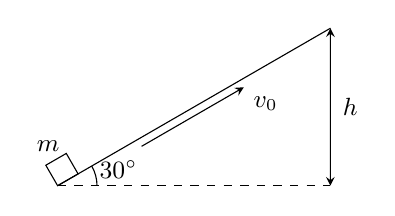
\begin{tikzpicture}
  \draw(0,0)--(30:4); 
  \draw[dashed](0,0)--(3.464,0);
  \draw [<->,>=stealth](3.464,0)--(30:4);
  \draw [rotate=30] (0,0) rectangle (0.3,0.3);
  \draw [rotate=30] (0.15,0.5) node {\small $m$};
  \draw (0:0.5) arc (0:30:0.5);
  \draw (15:0.8) node {\small $30^\circ$};
  \draw [->,>=stealth] (0.2,0)++(30:1)--++(30:1.5) node [anchor=north west] {\small $v_0$};
  \draw (3.5,1) node [anchor=west]{\small $h$};
\end{tikzpicture}
:>所示,绷紧的传送带在电动机带动下,始终保持$v_0=2m/s$的速度匀速运行,传送带与水平地面的夹角$\theta=30^\circ$,现把一质量$m=10kg$的工件轻轻地放在传送带底端,由传送带传送至$h=2m$的高处.已知工件与传送带间的动摩擦因数$\mu=\frac{\sqrt{3}}{2}$,$g$取$10m/s^2$.
[1]试通过计算分析工件在传送带上做怎样的运动?
[2]工件从传送带底端运动至$h=2m$高处的过程中摩擦力对工件做了多少功?

a.(1)工件先匀加速直线运动再匀速直线运动. \qquad (2) $220J$

e.(1)由于$\tan30^\circ<\mu$所以如果传送带足够长,则工件可以相对传送带静止而匀速运动,但是这不足以表明传送带是足够长的.我们来计算一下假如足够长,则匀加速过程可以使工件上升的高度$h'$由动能定理得
\[
  -mgh'+\mu mgh'\tan30^\circ =\frac{1}{2}mv_0^2-0
\]
解得
\[
  h'=\frac{v_0^2}{2g(\mu\cot30^\circ -1)}=0.4m
\]
由于$h'<h$所以工件先匀加速再匀速运动.

ee.(2)整个过程中,摩擦力由滑动摩擦力转变为静摩擦力,是一个变力,所以求它的功用动能定理比较方便.
\[
  -mgh+W_f=\frac{1}{2}mv_0^2-0
\]
解得
\[
  W_f=mgh+\frac{1}{2}mv_0^2=220J
\]

6.如<:
\begin{tikzpicture}
  \draw (180:1.5) arc (180:270:1.5);
  \draw (0,-1.5)--(3,-1.5);
  \draw (180:1.5) rectangle (-1.2,0.3);
  \draw[dashed](0,0)--(180:1.5) node [anchor=east]{\small $A$};
  \draw[dashed](0,0)--(0,-1.5) node [anchor=north]{\small $B$};
  \draw (2.5,-1.5) rectangle (2.8,-1.2);
  \draw (0,-0.7) node [anchor=west]{\small $R$};
\end{tikzpicture}
:>所示,$AB$为$1/4$圆弧轨道,半径为$R=0.8m$,$BC$是水平轨道,长$s=3m$,$BC$处的动摩擦因数为$\mu=\frac{1}{15}$,今有质量$m=1kg$的物体,自$A$点从静止起下滑到$C$点刚好静止.求物体在轨道$AB$段所受阻力对物体做的功.

a.-6J

e.从A到C由动能定理得
\[
  W_f-\mu mgs+mgR=0-0
\]
解得
\[
  W_f=\mu mgs-mgR=-6J
\]

7.一个物体从斜面上高$h$处由静止滑下并紧接着在水平面上滑行一段距离后停止,测得停止处对开始运动处的水平距离为$S$,如<:
\begin{tikzpicture}
  \draw [color=white,pattern=north west lines] (0,0) rectangle (2,-0.2); 
  \draw (0,0)--(2,0);
  \draw (0,0)--(150:1.5);
  \draw[rotate=150] (1.2,0) rectangle (1.5,-0.3);
  \draw[dashed](-1.5,0)--(0,0);
  \draw[<->,>=stealth](150:1.45)--(-1.2557,0);
  \draw (-1.3,0.35) node [anchor=east]{\small $h$};
  \draw[dashed] (1.7,0) rectangle (2,0.3);
  \draw[<->,>=stealth] (-1.2557,-0.4)--(2,-0.4);
  \draw (-1.2557,-0.1)--(-1.2557,-0.6);
  \draw (2,-0.1)--(2,-0.6);
  \draw (0.4,-0.8) node {\small $S$};
\end{tikzpicture}
:>所示,不考虑物体滑至斜面底端的碰撞作用,并设斜面与水平面对物体的动摩擦因数相同.求动摩擦因数$\mu$.

a.$\mu=\frac{h}{S}$

e.由动能定理得
\[
  mgh-\mu mgS=0
\]
解得
\[
  \mu=\frac{h}{S}
\]

ee.注意,此处摩擦力做的功等于$\mu mg$与水平方向距离的乘积,与斜面的夹角无关,设斜面底角为$\theta$,斜面长为$l$,则由正交分解可得摩擦力为$f=\mu mg\cos\theta$,于是摩擦力做功为
\[
  W_f=-\mu mg\cos\theta \cdot l
\]
由于$x=l\cos\theta$,所以有
\[
  W_f=-\mu mgx
\]
在本题中可以分为斜面和水平面二部分,则摩擦力做功为
\[
  W_f=-\mu mg x_1-\mu mgx_2=-\mu mgS
\]

8.从离地面$H$高处落下一个小球,小球在运动过程中所受的空气阻力是它重力的k($k<1$)倍,而小球与地面相碰后,能以相同大小的速率反弹,求:
[1]小球第一次与地面碰撞后,能够反弹的最大高度是多少?
[2]小球从释放开始,直到停止弹跳为止,所通过的总路程是多少?

a.(1)$\frac{1-k}{1+k}\cdot H$ \qquad (2) $S=\frac{H}{k}$

e.(1)如<:
\begin{tikzpicture}
  \draw (-1,0)--(1,0); 
  \draw [color=white,pattern=north west lines](-1,0) rectangle (1,-0.2);
  \draw[dashed] (-0.4,0)--(-0.4,2);
  \draw (-0.4,2.2) circle [radius=0.2];
  \draw[dashed] (0.4,0)--(0.4,1);
  \draw (0.4,1.2) circle [radius=0.2];
  \draw (-0.4,1) node [anchor=east]{\small $H$};
  \draw (0.4,0.5) node [anchor=west]{\small $h$};
\end{tikzpicture}
:>所示,设反弹的最大高度为$h$,则由动能定理得
\[
  mg(H-h)-kmg(H+h)=0-0
\]
解得
\[
  h=\frac{1-k}{1+k}\cdot H
\]

ee.(2)全过程由动能定理得
\[
  mgH-kmgS=0
\]
解得
\[
  S=\frac{H}{k}
\]

ee.第(2)问也可以借助{\bf 等比数列}直接求解.设第n次上升的高度为$H_n$,则由动能定理得
\[
  mg(H_n-H_{n+1})-kmg(H_n+H_{n+1})=0
\]
解得
\[
  \frac{H_{n+1}}{H_n}=\frac{1-k}{1+k}=q
\]
则前n项和为
\[
  S_n=H_0+2(H_1+H_2+\cdots +H_n)
\]
上式即
\[
  S_n=2H_0(1+q+q^2+\cdots+q^n)-H_0
\]
解得
\[
  S_n=2H_0\frac{1-q^{n+1}}{1-q}-H_0
\]
令$n\to\infty$得
\[
  S=\frac{2H_0}{1-q}-H_0
\]
代入$q=\frac{1-k}{1+k}$得
\[
  S=\frac{H_0}{k}
\]
在本题中$H=H_0$则
\[
  S=\frac{H}{k}
\]

\end{calculate}
